%% 内容梗概

%% プリアンブル %%%%%%%%%%%%%%%%%%%%%%%%%%%%%%%%%%%%%%%%%%%%%%%%%%%%%%%%
\documentclass[a4j]{jarticle}

\usepackage{kut-abstract}
\usepackage[dvips]{graphicx}
\usepackage{url}
\usepackage{here}
%% 表題 %%%%%%%%%%%%%%%%%%%%%%%%%%%%%%%%%%%%%%%%%%%%%%%%%%%%%%%%%%%%%%%%
%% 注意! 情報学群生の場合は,以下の \ScInfo を有効にすること.
\ScInfo        %% 情報学群生の場合

\Bachelor	%% 卒業研究論文梗概の場合
%\Project	%% プロジェクト研究報告書梗概の場合
%\Seminar	%% 特別研究セミナー課題研究報告書梗概の場合
%\Master	%% 修士学位論文(情報システム工学コース)梗概の場合
%\Doctorate	%% 博士学位論文(情報システム工学コース)梗概の場合
%\English	%% 英語の場合

\Eyears{2016}
\Etitle{English Title}
%\idnumber{}
\Eauthor{KAWAGUCHI, Takahiro}
\Eaffiliate{Yokoyama Lab.}

%% 本文 %%%%%%%%%%%%%%%%%%%%%%%%%%%%%%%%%%%%%%%%%%%%%%%%%%%%%%%%%%%%%%%%

\years{平成27}
\title{OpenStack環境でのオーケストレーション定義を容易にする\\GUIエディタの実現}
\idnumber{1160304}
\author{川口 ~~貴大}
\affiliate{分散処理OS研究室}

%% 本文 %%%%%%%%%%%%%%%%%%%%%%%%%%%%%%%%%%%%%%%%%%%%%%%%%%%%%%%%%%%%%%%%
\begin{document}
\begin{Abstract}
 
 \section{はじめに}
 OpenStackはOpenStackCommunityによって開発されたオープンソースのIaaS基盤ソフトウェアである.\cite{Document:1}
 
 OpenStackでは,複数のインスタンスやネットワークを一括起動するオーケストレーション機能がHeatにより提供されている.しかし,オーケストレーションを定義するテンプレートファイルは,記述に時間がかかり,また,記述ミスが起きやすい問題がある.
 
 \texttt 本研究ではGUIを用いたオーケストレーション定義エディタを実現し,短時間かつ容易に仮想環境を定義可能とした.
 \section{オーケストレーション定義エディタ}
 \subsection{問題点と要件}
 従来のHeatでは,テンプレートファイルをテキストエディタで記述する.そのため,「テンプレートファイルから構成情報を把握しづらい」,「テキスト記述量が膨大」,「テンプレートファイルの書式が複雑」,といった問題点がある.それらの問題点を解決するために以下方針でGUIを検討する.
 \begin{description}
 	\vspace{-2mm}
 	\item[(GUIを採用)]構築中のシステム構成を可視化
 	\vspace{-2mm}
 	\item[(手動入力を撤廃)]テキスト記述量を削減し,システム構築所要時間を短縮する.プルダウンメニューで記述内容を提供することによりテンプレートファイルの複雑な書式を意識することなく記述可能に.
 	\vspace{-2mm}
 	%\item[(Heat専門知識の排除)]学習コストの削減
 	%\vspace{-2mm}
 \end{description}
 \vspace{-5mm}
 \subsection{オーケストレーション定義エディタの概要}
 オーケストレーション定義エディタ(以下エディタ)では,構築中のシステム構成を可視化するためにGUIを採用している.エディタの概略図を図\ref{graf:1}に示す.
 \begin{figure}[H]
 	\begin{center}
 		\vspace{-5mm}
 		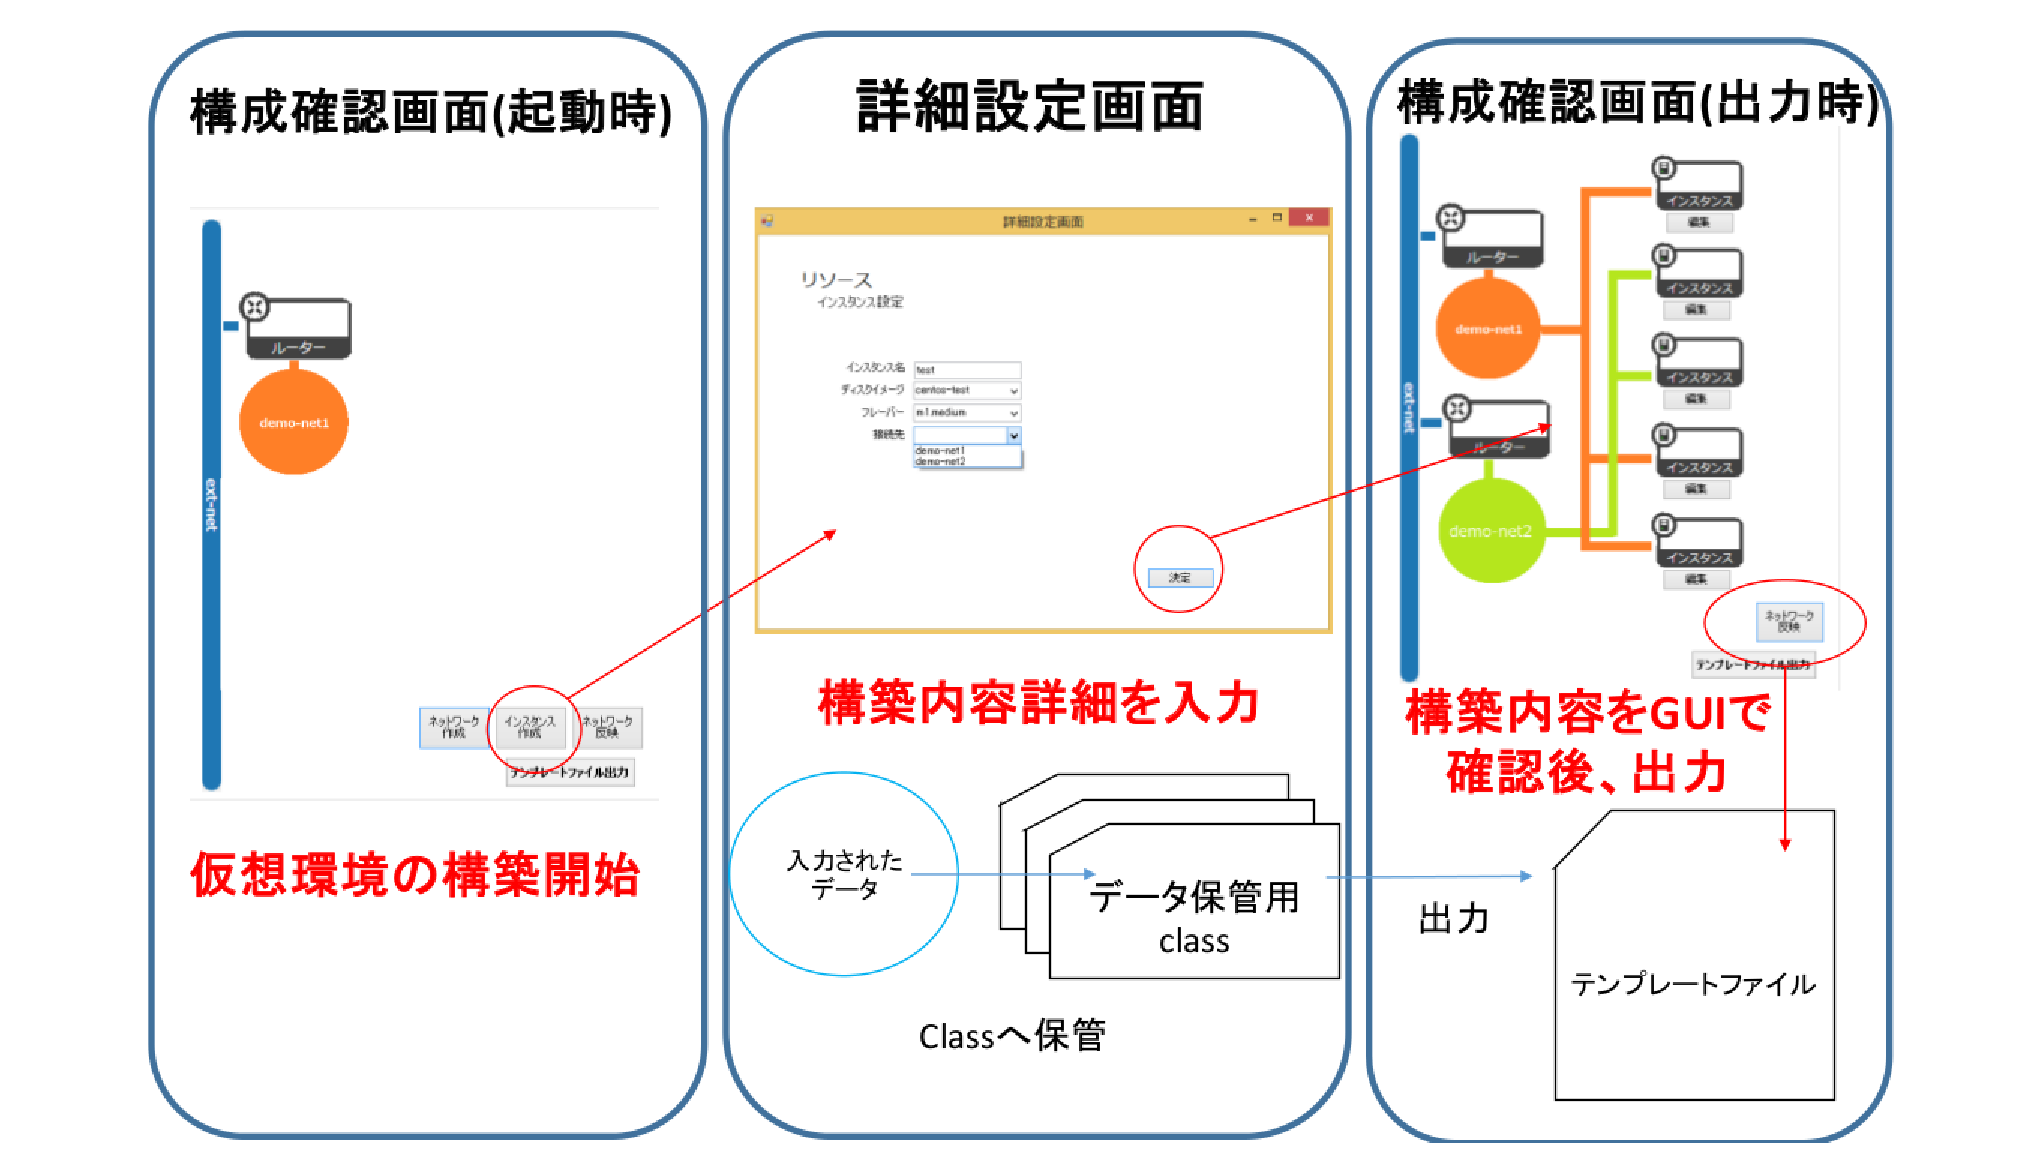
\includegraphics[scale=0.27]{Document/GUIEditorOverview.eps}
 		\caption{オーケストレーション定義エディタの概略}
 		\label{graf:1}
 	\end{center}
 \end{figure}
 \vspace{-8mm}
 
 テキスト入力を撤廃するために,入力される内容が決まっている項目は予め文字列データとして保存,出力時に自動でテンプレートファイルへ記述される.テンプレートファイル構築毎に入力内容が異なるものはプルダウンメニューで選択肢を用意,利用者に選択させ決定後テンプレートファイルへ出力する.これにより利用者は,Heat専門知識を意識することなくシステム構築が可能となった.
% \subsection{一部を除く手動入力項目の撤廃}
% オーケストレーション定義エディタでは従来方式の問題点のひとつであるテンプレートファイル作成時記述量の増加によるミスの改善,それに伴うテンプレートファイル作成所要時間を削減するために,インスタンス名入力項目以外の項目全てで手動入力方式を廃止,代わりにプルダウンメニューを採用した.これにより入力時間の大幅短縮,入力項目のエラー発生抑制を実現した.
% \begin{figure}[hbtp]
%  \begin{center}
%   \includegraphics[width=\columnwidth,clip]{im_outline}
%   \vspace{-2zh}
%   \caption{電子部品自動挿入機の概観}
%   \label{fig:im_outline}
%  \end{center}
% \end{figure}
% \vspace{-1zh}
% \begin{equation}
%  losstime = \sum_{i = 1}^{n - 1}l_{p(i) p(i + 1)} + l_{p(n) p(1)}
%   \label{eq:losstime}
% \end{equation}

 \section{評価}
 被験者5人が,従来方式とエディタそれぞれを使用して所定のシステム構成を構築,テンプレートファイル作成所要時間とエラー発生回数を計測した.3セグメント5インスタンス構成を構築した際の作成所要時間を図\ref{graf:2}に示す.
 \begin{figure}[H]
 	\begin{center}
 		\vspace{-4mm}
 		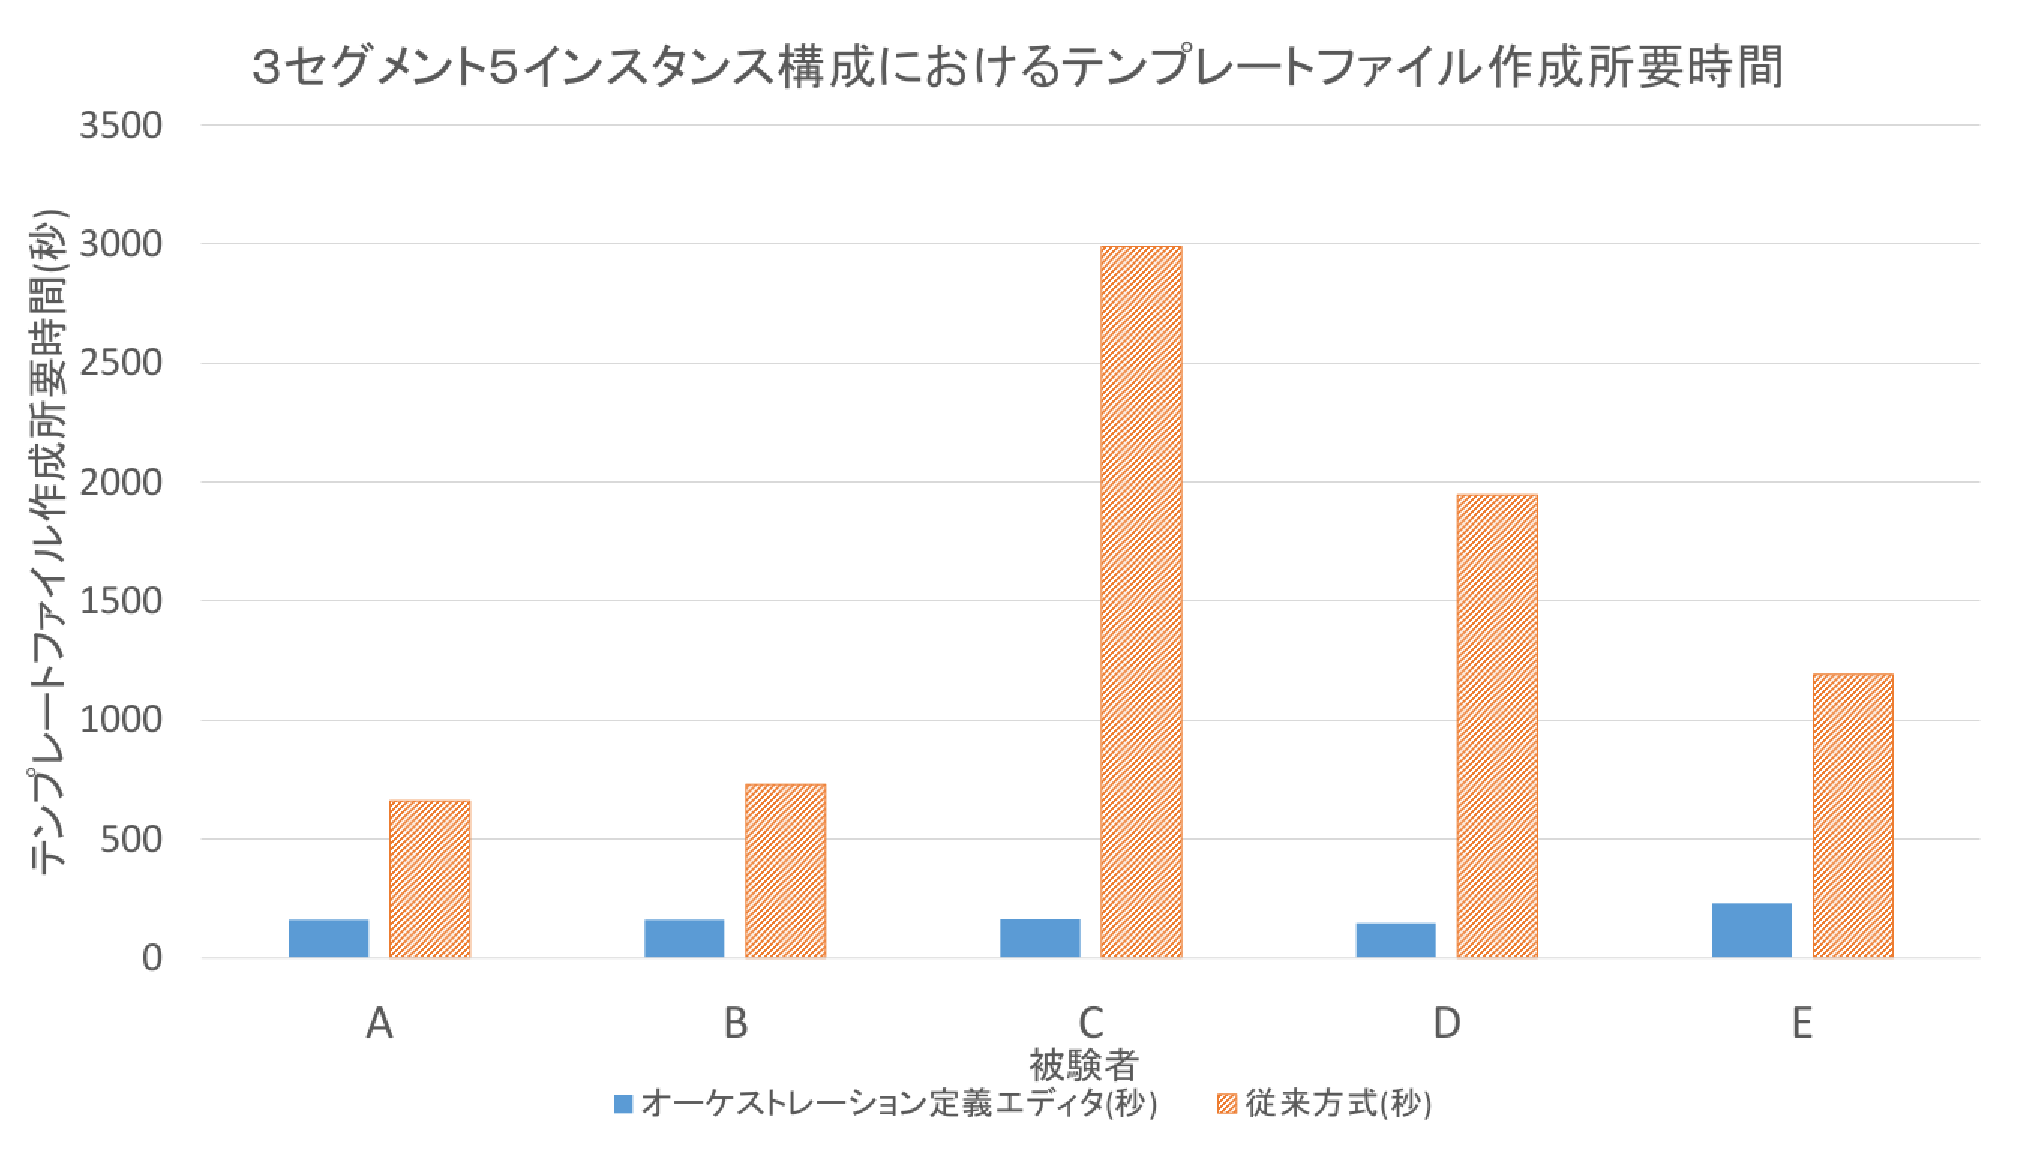
\includegraphics[scale=0.265]{Document/Abstract_Comparison.eps}
 		\caption{テンプレートファイル作成所要時間}
 		\label{graf:2}
 	\end{center}
 \end{figure}
 \vspace{-8mm}
 結果は,被験者全員手法に関する学習時間はエディタの学習時間が従来方式の学習時間よりも短くなった.また,テンプレートファイル作成所要時間は従来方式で作成所要時間に個人間でばらつきがあり尚且つ非常に長い時間がかかったが,エディタ使用時のテンプレートファイル作成所要時間は被験者間で所要時間に差は少なく且つ短時間で作成完了となった.
% \begin{itemize} \vspace*{-1zh}
%  \item 適応度比例戦略による複製 \vspace*{-1zh}
%  \item OX,PMX,CX という 3 種類の交叉 \vspace*{-1zh}
%  \item ランダムに選ばれた 2 点の遺伝子を交換する突然変異 \vspace*{-1zh}
%  \item 2-opt アルゴリズムによる部品挿入順序の局所最適化 \vspace*{-1zh}
% \end{itemize}
% という流れを繰り返す.
 
 \section{まとめ}
 本研究ではOpenStack内コンポーネントであるHeatを使用したシステム定義を記述する問題点である膨大な記述量と構築内容の把握しづらさを解決するためにオーケストレーション定義エディタを実現した.これにより従来方式よりテンプレートファイル作成所要平均時間を大幅短縮,構築内容もGUIにて可視化されより容易にHeatによるシステム構築を可能にした.
% \vspace{-2zh}
% \begin{table}[hbtp]
%  \begin{center}
%   \caption{実験結果}
%   \label{tab:result}
%   \begin{tabular}{|c|c||r|r|r|r|} \hline
%	\multicolumn{2}{|c||}{Data}	&
%	\multicolumn{2}{c|}{Prev.}	&
%	\multicolumn{2}{c|}{our method}	\\ \hline
%	部品数	& 品種数&
%	\multicolumn{1}{c|}{Best} & \multicolumn{1}{c|}{Time} &
%	\multicolumn{1}{c|}{Best} & \multicolumn{1}{c|}{Time}	\\ \hline\hline
%			& 10	& 10	&   250.0	&  2	&   48.5	\\ \cline{2-6}
%	\lw{100}& 20	& 30	&   336.2	& 16	&   70.5	\\ \cline{2-6}
%			& 30	& 50	&   347.1	& 40	&   98.7	\\ \cline{2-6}
%			& 40	& 66	&   363.3	& 58	&  168.4	\\ \hline
%			& 10	& 14	&  2346.3	&  0	&  196.8	\\ \cline{2-6}
%	\lw{200}& 20	& 36	&  2840.8	& 19	&  302.0	\\ \cline{2-6}
%	 		& 30	& 57	&  2770.0	& 38	&  578.9	\\ \cline{2-6}
%	 		& 40	& 87	&  3300.8	& 64	&  723.2	\\ \hline
%			& 10	&  6	&  8457.6	&  1	&  391.5	\\ \cline{2-6}
%	\lw{300}& 20	& 31	&  9938.1	& 12	&  724.7	\\ \cline{2-6}
%	 		& 30	& 58	& 11092.8	& 31	& 1309.5	\\ \cline{2-6}
%	 		& 40	& 89	& 12345.4	& 51	& 1577.2	\\ \hline
%   \end{tabular}
%  \end{center}
% \end{table}
% \vspace{-2zh}
 
%% 参考文献 %%%%%%%%%%%%%%%%%%%%%%%%%%%%%%%%%%%%%%%%%%%%%%%%%%%%%%%%%%%%
\begin{thebibliography}{99}
 \bibitem{Document:1} OpenStack,\url{https://www.openstack.org/}
\end{thebibliography}

\end{Abstract}
\end{document}
